\begin{frame} \frametitle{\vspace*{0.5cm}Results: Early evolution of the interface}
  \vspace*{-0.25cm}%
  \hspace*{0.03\textwidth}%
  \begin{minipage}{0.2\linewidth}
    \hfill%
    \begin{figure}
      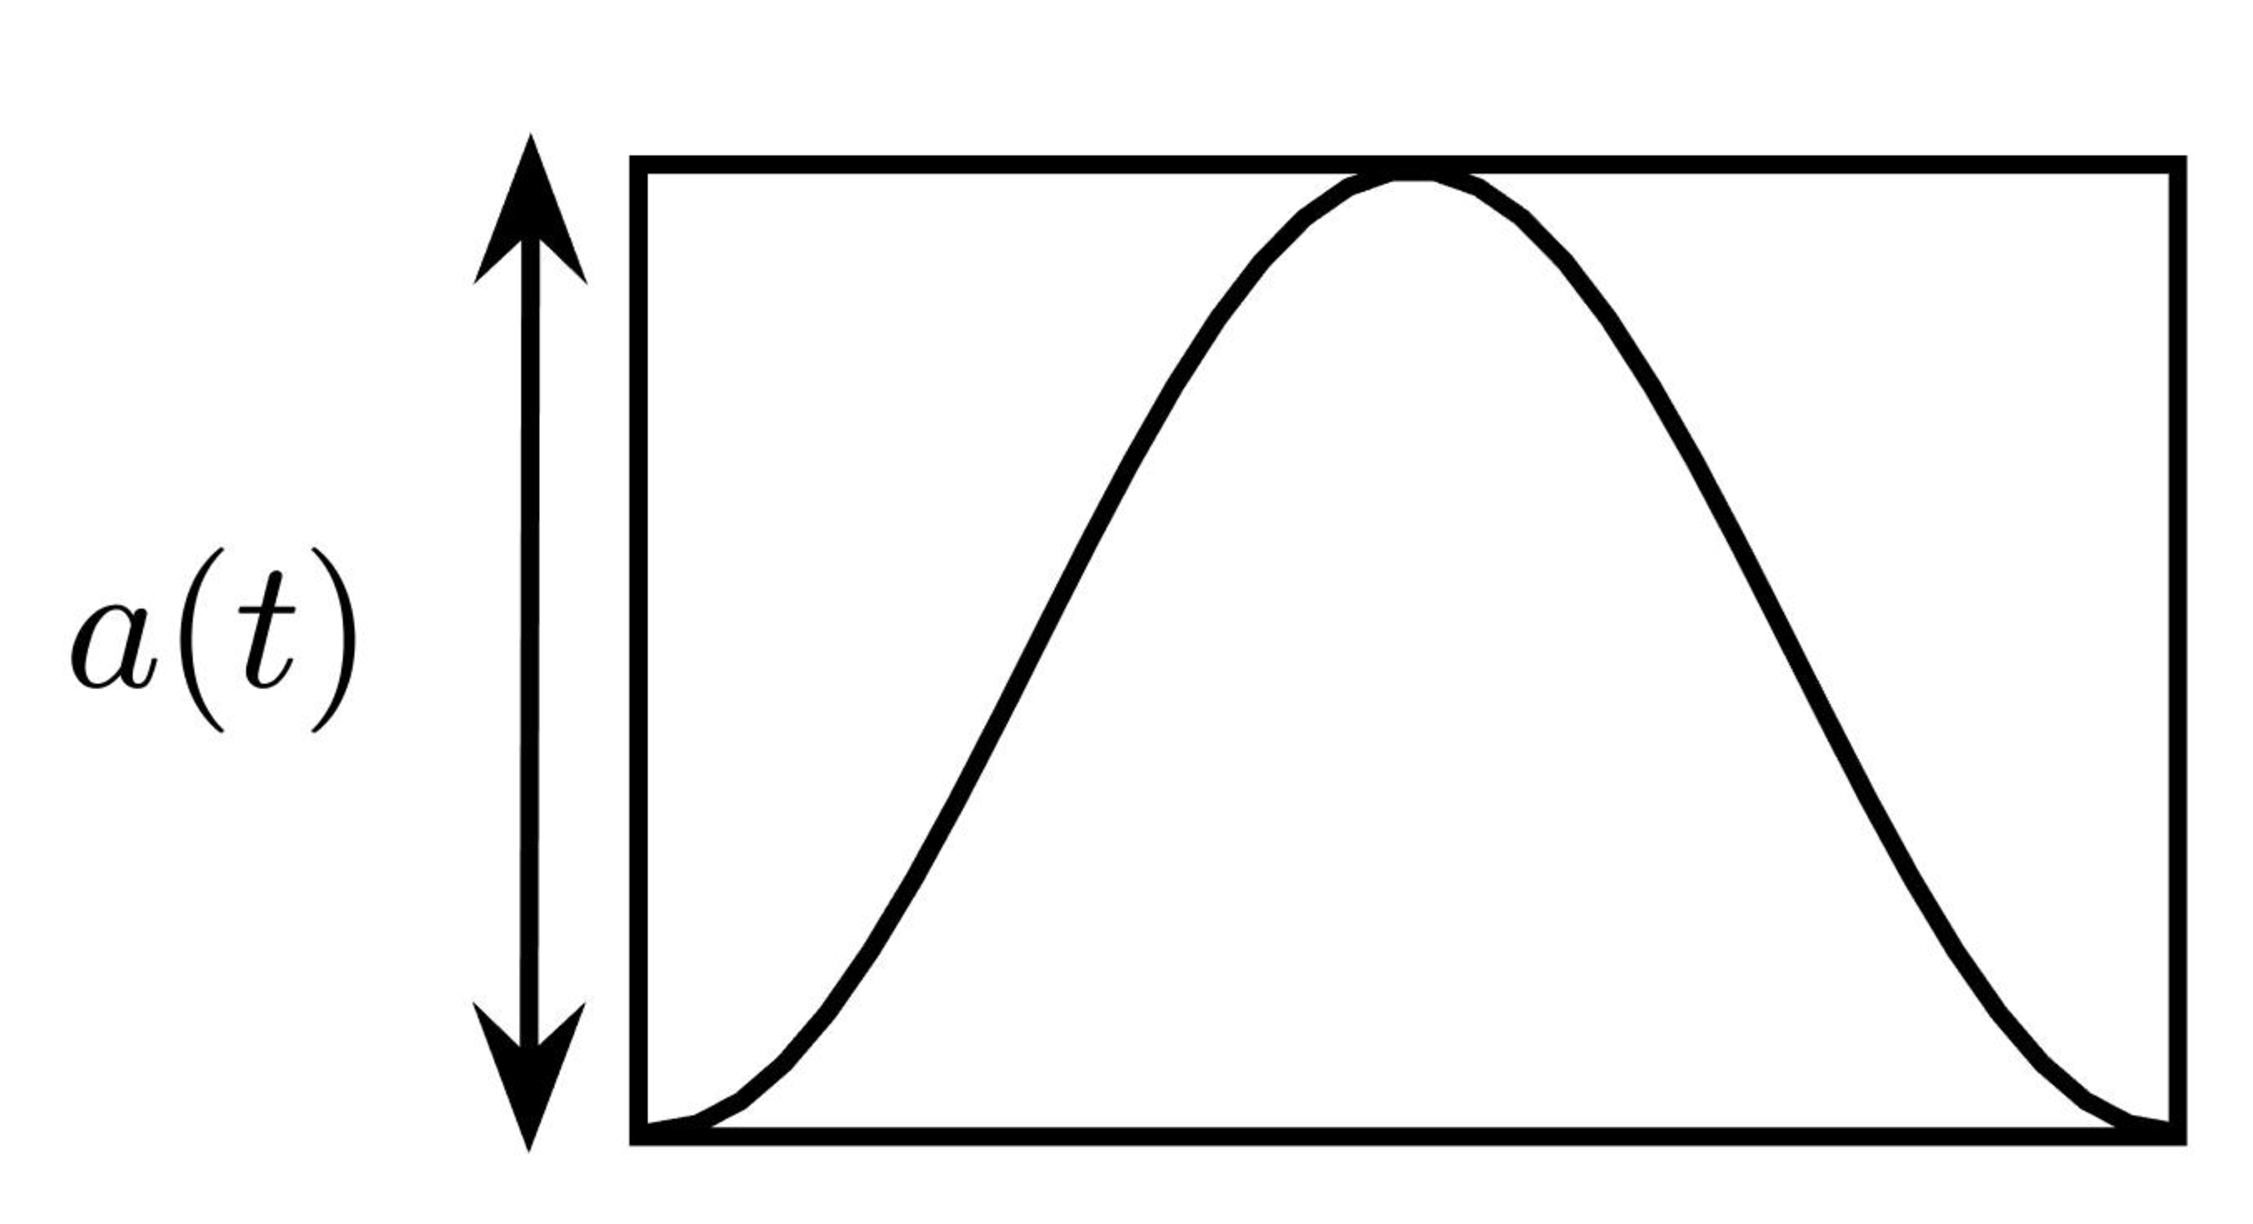
\includegraphics[height=0.18\textheight]{../figs/lung_figs/a0_schematic}%
    \end{figure}
  \end{minipage}\begin{figure}
    \hfill%
    \centering
    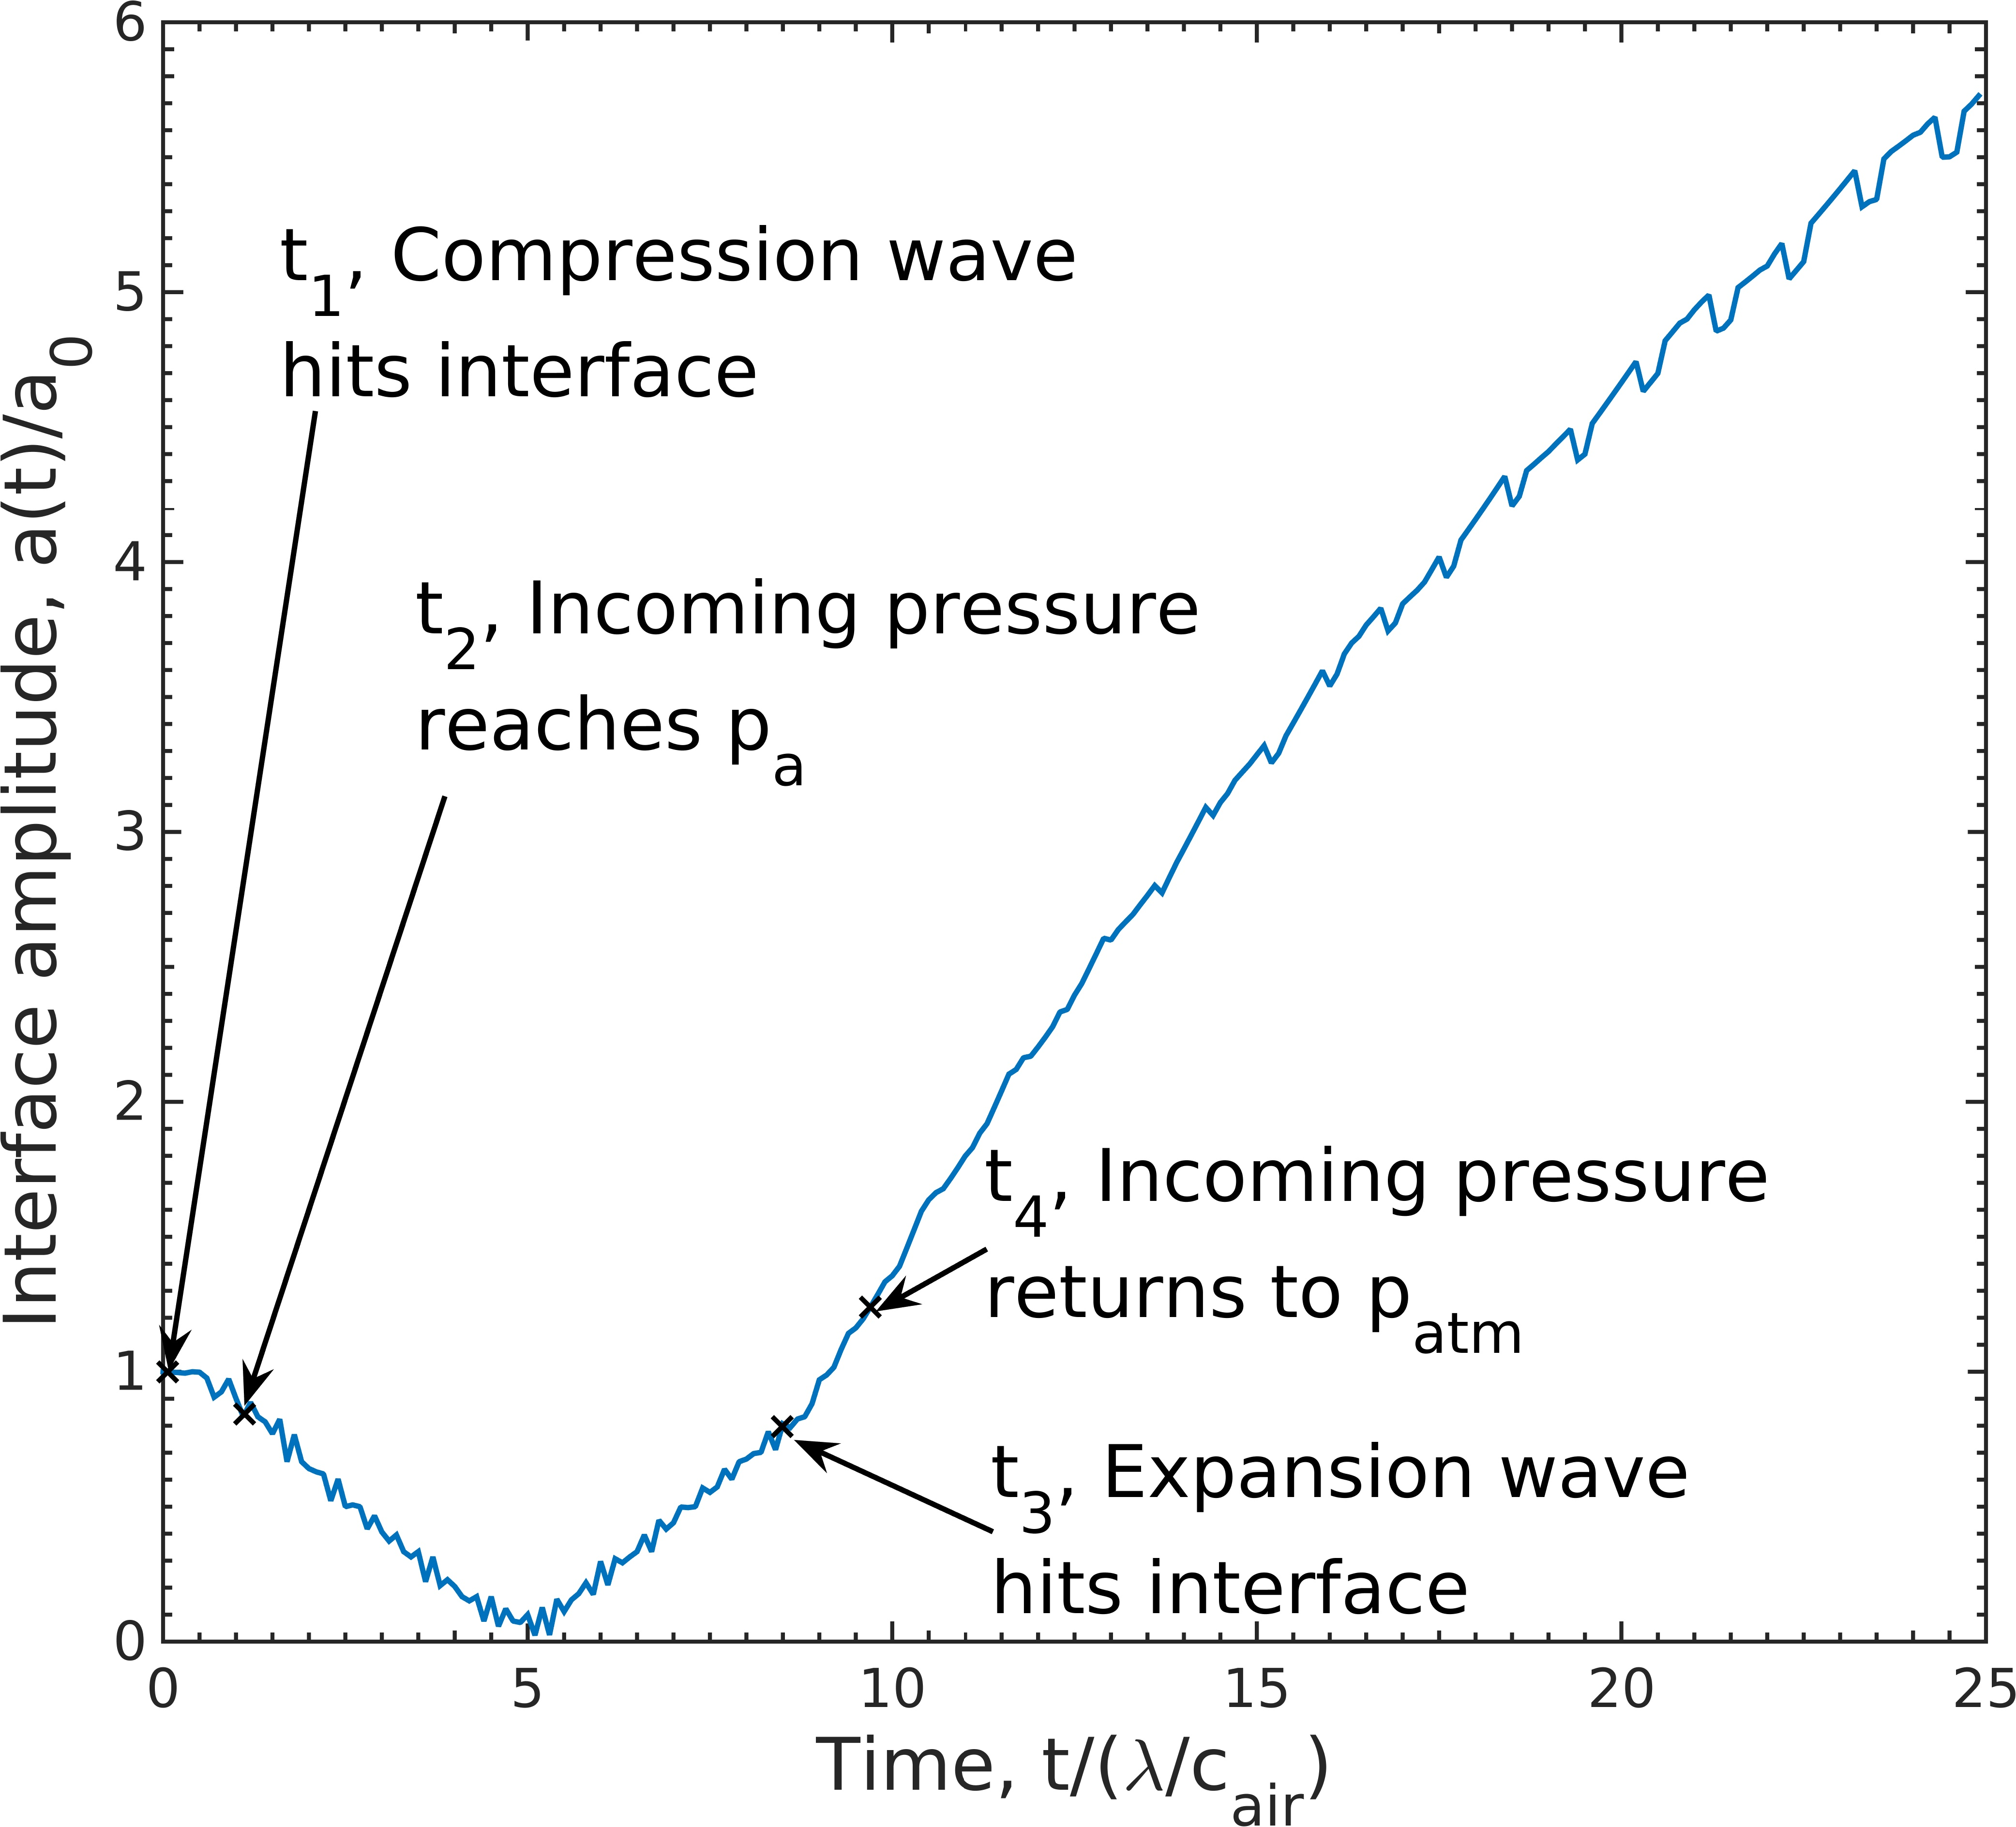
\includegraphics[height=0.5\textheight]{../figs/lung_figs/trapz10_intf_schematic}%
    \hfill%
    % 
    \begin{tikzpicture}%
      \node[anchor=south west,inner sep=0] (image) at (0,0) {%
        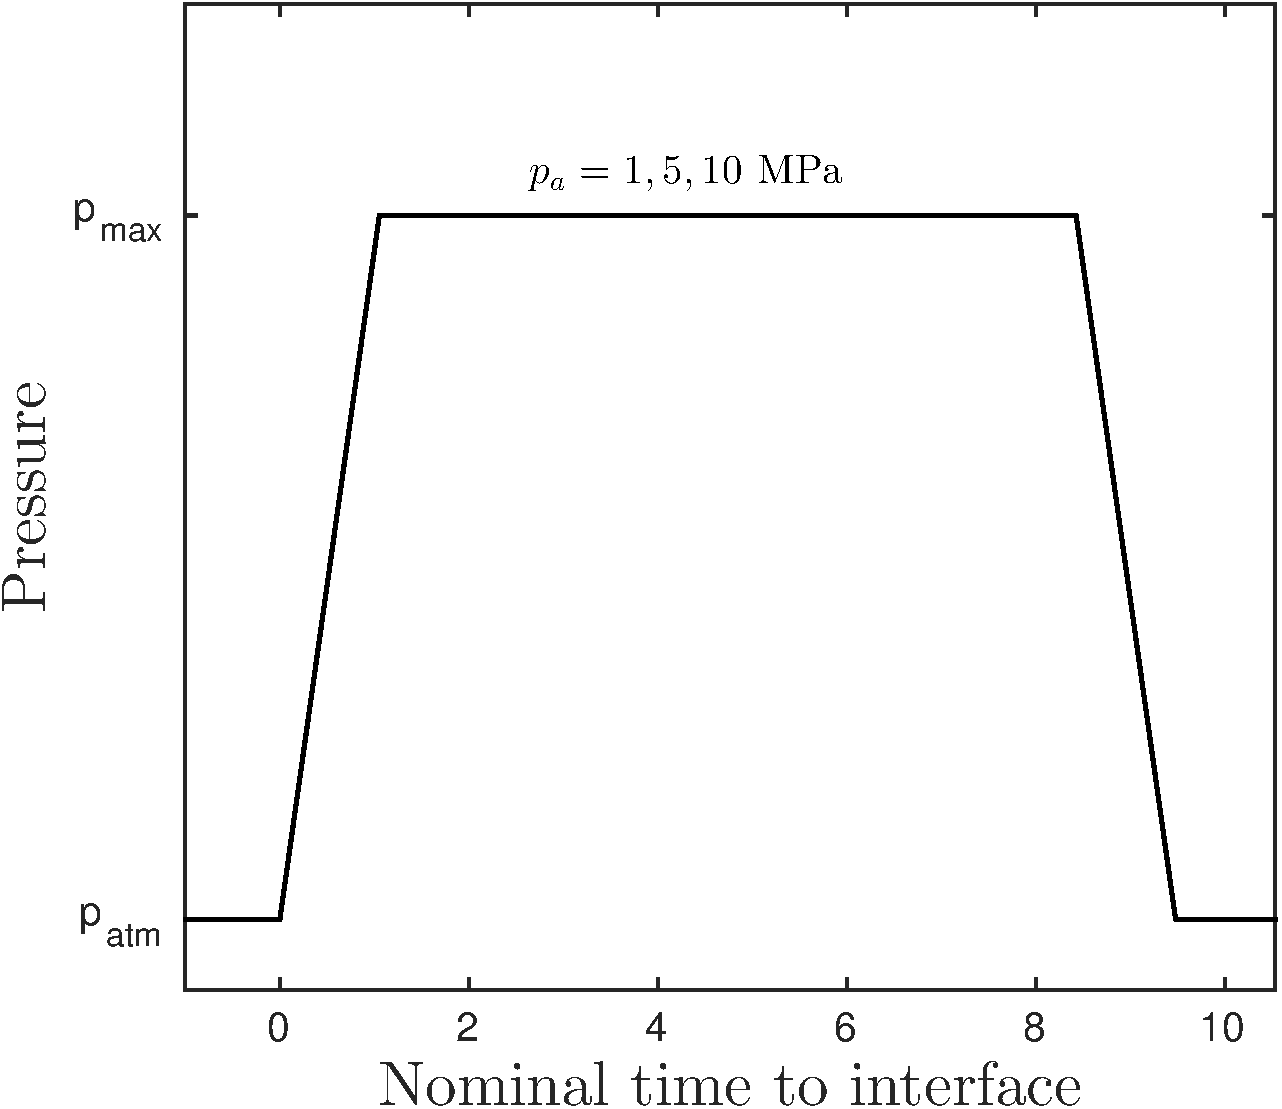
\includegraphics[height=0.5\textheight]{../figs/lung_figs/p0_vs_t_nd.pdf}%
      };%  
      \begin{scope}[x={(image.south east)},y={(image.north west)}]%
        \node[font=\footnotesize,right] at (0.22,0.18){ $t_1$};%
        \node[font=\footnotesize,right] at (0.22,0.8){ $t_2$};%
        \node[font=\footnotesize,right] at (0.83,0.8){ $t_3$};%
        \node[font=\footnotesize,right] at (0.82,0.18){ $t_4$};%
      \end{scope}%  
    \end{tikzpicture}%
    \hfill%
    % 
  \end{figure}
  \vfill%
  The interface perturbation is initially compressed $(0^+\leq t\leq5)$, experiences a phase change $(t=5)$, then grows $t>5$.%
  \vfill%
  \note{
    \begin{enumerate}
    \item If we look at the peak-to-peak amplitude of the interface
      perturbation as a function of time, we can see that early own
      the interface compresses slightly during the compression wave
    \item Then continues to compress until inverting phase at $t=5$.
    \item After the phase inversion, the expansion occurs.
    \item And the interface continues growing long after the wave has completely left.
    \end{enumerate}
  }
\end{frame}
%%% Local Variables:
%%% mode: latex
%%% TeX-master: "../main"
%%% End:
